\begin{figure}
    \centering
    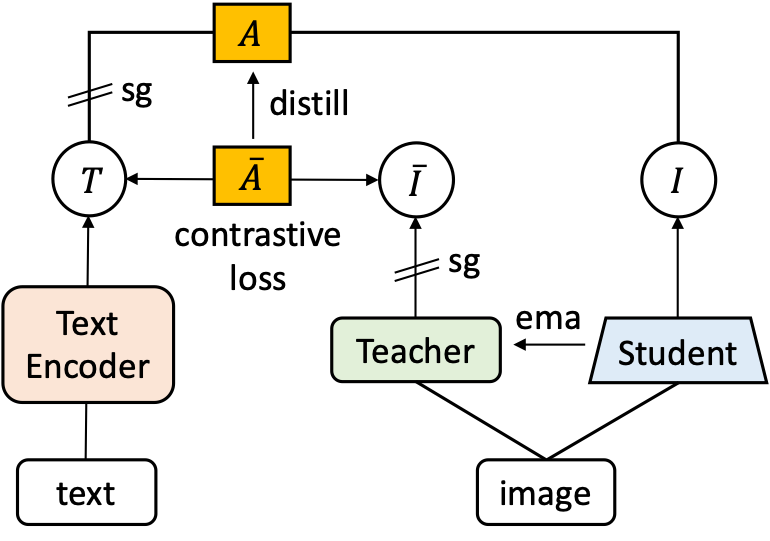
\includegraphics[width=0.8\columnwidth]{figures/imgs/figure_overview.png}
    \vspace{0.7em}
    \caption{Overview of ECLIPSE. Student encoder is trained to estimate the soft alignment matrix $\bar{A}$ predicted by Text Encoder and the Teacher network.
    sg stands for stop-gradient, $I$ and $\bar{I}$ are encoded image with student and teacher network, respectively.
    }
    \label{fig:fig_overview}
\end{figure}